\chapter{Market Research: TAM, SAM, and SOM}
\label{ch:market-research}

\section*{How to read this chapter}

This chapter carries two registers that must not be blurred together. The first is the near-term reality and the ask: Devorix is pre-launch, pre-revenue, with zero advertisers signed, zero installs, a solo founder, and a \textrm{\textrupee}1 lakh total budget. The numbers that matter for the funding conversation today are the locked four-month plan and the go/no-go gate it feeds (MASTER-PLAN \S 8.3). This is a pre-seed / accelerator-stage story --- ``give us a small check or a slot to prove the loop works'' --- not a seed-round forecast.

The second register is the long-term vision, clearly labeled as vision. The TAM ceiling math and the agentic-economy market context are \emph{optionality and direction}, not the thing being underwritten. They answer ``why is this infrastructure bet worth taking if the near-term loop works,'' not ``fund our billion-dollar projection.''

Every figure in this chapter carries one of three labels, used consistently and never blurred through synthesis:

\begin{itemize}
  \item \textit{[Verified fact]} --- named, on-record, or independently multi-sourced.
  \item \textit{[Industry estimate]} --- published by research firms or third parties, directionally consistent but without a single authoritative number.
  \item \textit{[Internal assumption]} --- Devorix's own model output or extrapolation; not a researched fact.
\end{itemize}

No locked decision (50/50 revenue split, \textrm{\textrupee}300 payout threshold, hybrid pricing ladder, 5-second impression, \textrm{\textrupee}94 FX, India-first / Global-Phase-2) is reopened here. All locked numbers are carried forward as given.

\section{A reconciliation note on adoption-share figures}
\label{sec:adoption-reconciliation}

Two of our inputs carry different numbers for Claude Code / Cursor adoption, and rather than silently dropping either, we resolve the discrepancy explicitly here.

MASTER-PLAN \S 10 states that ``Cursor and Claude Code are tied at 18\% workplace usage each'' \textit{[Verified fact --- high confidence, converging independent surveys]} \cite{masterplan_2026}. A more recent 2026 survey aggregation, by contrast, reports that among agentic-tool users specifically, the primary-tool split is Claude Code 28\% / Cursor 24\% \textit{[Industry estimate --- single aggregation source]} \cite{agentictoolsurvey_2026}.

\textbf{These are not contradictory --- they measure different things.} The 18\%/18\% figure is workplace usage of any kind across the whole developer population; the 28\%/24\% figure is primary-tool selection among the subset who already use agentic tools regularly. A higher number on a narrower, more-engaged base is exactly what one would expect.

\textbf{Decision for this PRD:} we use 18\% workplace usage (MASTER-PLAN \S 10) as the headline adoption anchor, because it is the better-sourced, more conservative figure, and because it matches the convention used everywhere else in the plan. We carry the 28\%/24\% primary-tool split forward as a directional, favorable signal for Claude Code's momentum (consistent with the ``\$0 \(\to\) \$2.5B Claude Code run-rate in 9 months'' data point) --- \emph{not} as a planning number.

\textbf{Flag for the next funding conversation:} the 28\%/24\% figure should be re-verified against a second independent source before being quoted to an investor. It currently rests on a single 2026 aggregation. It is recorded here, not dropped.

\section{Top-down: adjacent market anchors}
\label{sec:top-down}

None of the markets below measure Devorix's niche --- wait-state sponsorship on AI coding tools --- directly. They establish that the surrounding dollar pools are large and real. They cannot be divided down to produce a credible Devorix TAM; that is a genuine gap, flagged in Section~\ref{sec:open-questions-market}.

\begin{table}[htbp]
\centering
\caption{Adjacent market anchors (top-down, scale context only)}
\label{tab:adjacent-markets}
\small
\begin{tabular}{p{4.0cm}p{5.3cm}p{3.0cm}}
\toprule
\textbf{Market} & \textbf{Size} & \textbf{Label} \\
\midrule
AI code tools market (narrow def.) & \$9.35B (2026); \$7.65B (2025) \(\to\) \$9.46B (2026) across firms & \textit{Industry estimate} \cite{aicodetools_2026} \\
AI code tools market (broad def., incl. review/testing/platforms) & \$29.47B (2025) \(\to\) \$34.58B (2026) & \textit{Industry estimate} (wide range reflects category-boundary disagreement) \cite{aicodetoolsbroad_2026} \\
Enterprise AI coding agents (Gartner) & \textasciitilde\$9.8--11.0B annualized (Apr 2026) & \textit{Verified fact} \cite{gartner_2026} \\
Claude Code run-rate (Devorix's first target tool) & \$0 \(\to\) \$2.5B run-rate in 9 months & \textit{Verified fact} (total tool revenue, \emph{not} an ad-monetization figure) \cite{anthropic_2026} \\
Cursor (Anysphere) & \textasciitilde\$2B annualized rev., 1M+ paying customers, \$29.3B valuation (Nov 2025) & \textit{Verified fact} (named funding sources) \cite{anysphere_2025} \\
Developer tools market, global & \$7.44--8.8B (2026) \(\to\) \$15.72B by 2031 (\textasciitilde16\% CAGR) & \textit{Industry estimate} --- closest ``category'' anchor to Devorix's surface \cite{devtoolsmarket_2026} \\
Affiliate marketing, global (closest business-model analogue) & \$20.07B (2026) \(\to\) \$82.64B (2035) at 15.2\% CAGR; alt.\ \textasciitilde\$23.84B (2026) platform-layer only & \textit{Industry estimate} --- no developer-focused sub-segment isolated by any source \cite{affiliatemarketing_2026} \\
Agentic commerce / agent economy by 2030 & \$3--5T (McKinsey); narrower cuts \$190--500B (Morgan Stanley / Bain, US only) & \textit{Industry estimate} --- long-range, \textbf{not} a near-term TAM \cite{mckinsey_2026} \\
Dev-ad-platform benchmarks & daily.dev \$5,000--15,000/mo minimum spend, CPM \$10--20; SaaS spend \textasciitilde8\% of ARR on marketing & \textit{Industry estimate} --- sanity check: Devorix Tier-0 \textrm{\textrupee}10--15k/mo (\textasciitilde\$120--180) is far below the cheapest mainstream dev-ad minimum \cite{dailydev_2026} \\
\bottomrule
\end{tabular}
\end{table}

\textbf{Top-down read:} the correct top-down framing is narrow. Devorix competes for a slice of the dev-marketing budgets that already exist (\$5k--15k+/mo per advertiser on Carbon Ads, daily.dev, and dev newsletters today). The developer-tools market (\$7.4--8.8B, 2026) and the dev-marketing-spend layer on top of it are the right-order-of-magnitude pools Devorix's advertiser revenue is drawn from --- \textbf{not} the multi-trillion agentic-commerce figures, which are vision-context only.

\begin{figure}[htbp]
\centering
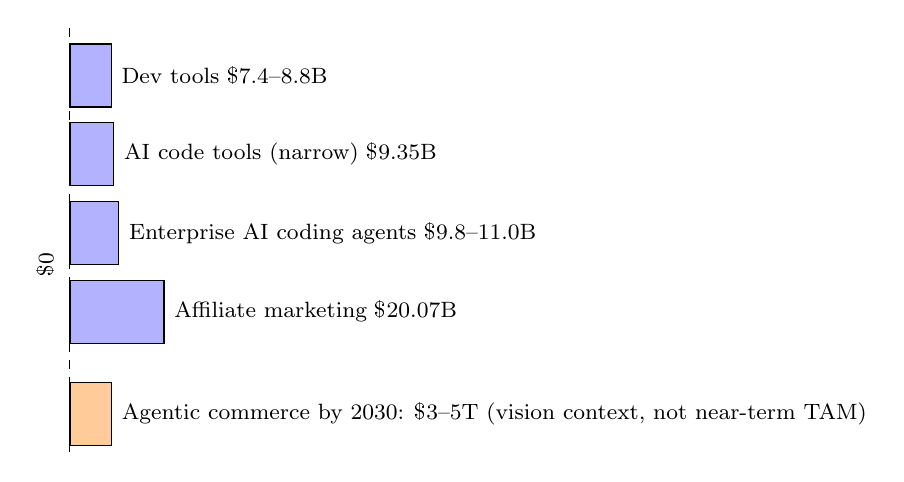
\begin{tikzpicture}[
  every node/.style={font=\small},
  bar/.style={draw, fill=blue!30, minimum height=0.8cm},
  visionbar/.style={draw, fill=orange!40, minimum height=0.8cm}
]
\def\scale{0.0017}
\node[bar, minimum width=8.8*\scale*1000, anchor=west] (b1) at (0,0) {};
\node[anchor=west, font=\footnotesize] at (b1.east) {Dev tools \$7.4--8.8B};

\node[bar, minimum width=9.35*\scale*1000, anchor=west] (b2) at (0,-1) {};
\node[anchor=west, font=\footnotesize] at (b2.east) {AI code tools (narrow) \$9.35B};

\node[bar, minimum width=10.4*\scale*1000, anchor=west] (b3) at (0,-2) {};
\node[anchor=west, font=\footnotesize] at (b3.east) {Enterprise AI coding agents \$9.8--11.0B};

\node[bar, minimum width=20.07*\scale*1000, anchor=west] (b4) at (0,-3) {};
\node[anchor=west, font=\footnotesize] at (b4.east) {Affiliate marketing \$20.07B};

\node[visionbar, minimum width=15, anchor=west] (b5) at (0,-4.3) {};
\node[anchor=west, font=\footnotesize] at (b5.east) {Agentic commerce by 2030: \$3--5T (vision context, not near-term TAM)};

\draw[dashed] (0,0.6) -- (0,-4.8);
\node[font=\footnotesize, rotate=90] at (-0.3,-2.4) {\$0};
\end{tikzpicture}
\caption{Adjacent-market scale comparison (top-down anchors). The agentic-commerce figure is drawn at a compressed, visually distinct scale and flagged as vision context, not a near-term TAM input.}
\label{fig:adjacent-markets}
\end{figure}

\section{Bottom-up: India developer base to realistic capture}
\label{sec:bottom-up}

\begin{table}[htbp]
\centering
\caption{Bottom-up funnel: India developer base to agentic-tool pool}
\label{tab:bottom-up-funnel}
\small
\begin{tabular}{p{4.3cm}p{5.0cm}p{3.2cm}}
\toprule
\textbf{Step} & \textbf{Figure} & \textbf{Label} \\
\midrule
India developers on GitHub, 2026 & \textbf{27 million} (up from 21.9M Oct 2025; 2M+ added in 2026) & \textit{Verified fact} (GitHub COO Kyle Daigle, multi-source) \cite{github_2026} \\
India developers on GitHub, 2030 projection & \textbf{57.5 million} (projected largest GitHub community globally) & \textit{Verified fact} (Satya Nadella, on record) \cite{nadella_2026} \\
Developers using any AI coding tool & 85--92\% global; India \textgreater 97\% have used, \textgreater 80\% regular use (among highest of any region) & Global = \textit{Verified fact} \cite{masterplan_2026}; India-specific = \textit{Industry estimate} \\
Using AI coding agents specifically (Devorix's actual surface) & Global \textasciitilde 55\% of devs regularly use AI agents; primary-tool split Claude Code 28\% / Cursor 24\% (see \S\ref{sec:adoption-reconciliation}) & \textit{Industry estimate} --- agentic use \(\neq\) autocomplete; Copilot's broad 58\% ``any-use'' is mostly autocomplete \cite{agentictoolsurvey_2026} \\
Implied India agentic-tool pool, 2026 & Working range \textbf{5--15M} (applying global \textasciitilde 55\% to 27M base; conservative cut for India's newer agentic penetration) & \textbf{\textit{Internal assumption}} --- built by applying a global ratio to the India base; no India-specific agentic-only survey exists \\
\bottomrule
\end{tabular}
\end{table}

\textbf{A deliberately conservative SAM stance:} the 5--15M range above is the outer envelope. MASTER-PLAN \S 3's more conservative ``single-digit millions'' framing is the safer planning assumption until India-specific primary research exists (an open question, Section~\ref{sec:open-questions-market}). We adopt single-digit-millions as the working SAM and treat 5--15M as the ceiling, not the plan.

\begin{figure}[htbp]
\centering
\begin{tikzpicture}[
  every node/.style={font=\small},
  dot/.style={draw, circle, fill=blue!20, minimum size=8mm},
  lbl/.style={font=\footnotesize}
]
\draw[-{Stealth[length=3mm]}, thick] (0,0) -- (10,0);
\foreach \x/\y in {0/2025.8, 2.5/2026, 8.5/2030} {
  \draw (\x,0.12) -- (\x,-0.12);
}
\node[dot, minimum size=10mm] at (0,0) {};
\node[lbl, above=2mm of {(0,0.4)}] at (0,1.0) {21.9M};
\node[lbl] at (0,-0.9) {Oct 2025};

\node[dot, minimum size=12mm, fill=blue!35] at (2.5,0) {};
\node[lbl] at (2.5,1.0) {27M};
\node[lbl] at (2.5,-0.9) {2026};

\node[dot, minimum size=18mm, fill=orange!40] at (8.5,0) {};
\node[lbl] at (8.5,1.4) {57.5M};
\node[lbl] at (8.5,-0.9) {2030};
\node[lbl, font=\scriptsize\itshape] at (8.5,-1.4) {(projection --- Nadella)};
\end{tikzpicture}
\caption{India developer population on GitHub: growth trajectory. 2030 figure is a projection, not a measured value.}
\label{fig:india-dev-growth}
\end{figure}

\section{Adoption split (cross-referenced)}
\label{sec:adoption-split}

\begin{figure}[htbp]
\centering
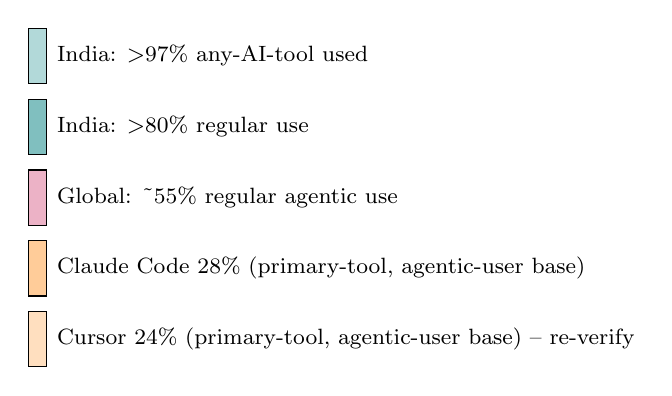
\begin{tikzpicture}[
  every node/.style={font=\small},
  hbar/.style={draw, fill=teal!30, minimum height=0.7cm},
]
\def\scl{0.06}
\node[hbar, minimum width=97*\scl, anchor=west] (r1) at (0,0) {};
\node[anchor=west, font=\footnotesize] at (r1.east) {India: \textgreater 97\% any-AI-tool used};

\node[hbar, minimum width=80*\scl, anchor=west, fill=teal!50] (r2) at (0,-0.9) {};
\node[anchor=west, font=\footnotesize] at (r2.east) {India: \textgreater 80\% regular use};

\node[hbar, minimum width=55*\scl, anchor=west, fill=purple!30] (r3) at (0,-1.8) {};
\node[anchor=west, font=\footnotesize] at (r3.east) {Global: \textasciitilde 55\% regular agentic use};

\node[hbar, minimum width=28*\scl, anchor=west, fill=orange!40] (r4) at (0,-2.7) {};
\node[anchor=west, font=\footnotesize] at (r4.east) {Claude Code 28\% (primary-tool, agentic-user base)};

\node[hbar, minimum width=24*\scl, anchor=west, fill=orange!25] (r5) at (0,-3.6) {};
\node[anchor=west, font=\footnotesize] at (r5.east) {Cursor 24\% (primary-tool, agentic-user base) -- re-verify};
\end{tikzpicture}
\caption{Adoption split across measurement bases. Rows 4--5 (primary-tool split, 28\%/24\%) are flagged for re-verification against a second source; see the note below.}
\label{fig:adoption-split}
\end{figure}
{\small\itshape Note: MASTER-PLAN \S 10 anchors workplace usage at 18\% each for Claude Code and Cursor, measured across the whole developer population rather than the agentic-user subset shown above. See Section~\ref{sec:adoption-reconciliation} for the full reconciliation.\par}

\section{TAM / SAM / SOM, stated explicitly}
\label{sec:tam-sam-som}

\begin{table}[htbp]
\centering
\caption{TAM / SAM / SOM definitions and figures}
\label{tab:tam-sam-som}
\small
\begin{tabular}{p{1.4cm}p{4.6cm}p{4.0cm}p{2.6cm}}
\toprule
\textbf{Layer} & \textbf{Definition} & \textbf{Figure} & \textbf{Label} \\
\midrule
TAM & All global developers using agentic AI coding tools, if a wait-state sponsorship layer existed for all of them at the locked Tier-1 Global CPM (\$5--8) & Not sized by any research firm. Back-of-envelope plausibly yields \textbf{low-to-mid hundreds of millions of USD/year} at full penetration and full fill & \textbf{\textit{Internal assumption}} --- weakest-grounded figure in this chapter; illustrative ceiling only \\
SAM & India developers using agentic AI coding tools (Claude Code first) who could realistically install a status-bar sponsor client & \textbf{Single-digit millions} (working); \textbf{5--15M} outer envelope & \textbf{\textit{Internal assumption}} --- intentionally wide given data gaps \\
SOM & Devorix's actual installs \(\times\) actual advertiser revenue, conditional on clearing the month-4 gate & M4 (locked): 500 installs, 3 advertisers, \textrm{\textrupee}45,000/mo. M24 (``likely''): \textasciitilde 5,000--9,000 installs, 6--10 advertisers, \textasciitilde\textrm{\textrupee}150,000--300,000/mo & \textbf{\textit{Internal assumption}} --- even the upper end is well under 1\% of SAM \\
\bottomrule
\end{tabular}
\end{table}

\textbf{The single most important structural insight}, carried from MASTER-PLAN \S 4/\S 11 and quantified here: the funnel from TAM to SOM does \emph{not} narrow primarily on the developer/supply side. 27M India GitHub developers is abundant and cheap to reach. The binding constraint is \textbf{advertiser demand} --- and that variable has no market-sizing number yet, because no one in this \textasciitilde 2.5-week-old category has found it. A TAM/SAM/SOM table built only on developer counts overstates how market-size-derived this business is. Devorix's near-term opportunity is \textbf{advertiser-revenue-constrained, not developer-supply-constrained}.

\begin{figure}[htbp]
\centering
\begin{tikzpicture}[every node/.style={font=\small}]
\draw[fill=blue!10, draw=blue!40] (0,0) circle (4.2);
\node[font=\footnotesize\bfseries, blue!70!black] at (0,3.6) {TAM};
\node[font=\scriptsize, align=center] at (0,3.0) {Low-to-mid hundreds};
\node[font=\scriptsize, align=center] at (0,2.65) {of \$M/yr (illustrative)};

\draw[fill=blue!25, draw=blue!50] (0,-0.6) circle (2.6);
\node[font=\footnotesize\bfseries, blue!80!black] at (0,1.55) {SAM};
\node[font=\scriptsize, align=center] at (0,1.05) {Single-digit millions};
\node[font=\scriptsize, align=center] at (0,0.72) {India agentic devs};
\node[font=\scriptsize, align=center] at (0,0.40) {(5--15M ceiling)};

\draw[fill=orange!50, draw=orange!70!black] (0,-1.6) circle (0.95);
\node[font=\footnotesize\bfseries, white] at (0,-1.6) {SOM};

\node[font=\scriptsize, align=left, anchor=west] at (4.6,-1.6) {M4: 500 installs / 3 advertisers};
\node[font=\scriptsize, align=left, anchor=west] at (4.6,-2.0) {/ \textrm{\textrupee}45,000/mo};
\node[font=\scriptsize, align=left, anchor=west] at (4.6,-2.6) {M24 likely: \textasciitilde 5,000--9,000 installs};
\node[font=\scriptsize, align=left, anchor=west] at (4.6,-3.0) {/ 6--10 advertisers / \textrm{\textrupee}150k--300k/mo};

\draw[-{Stealth[length=2.5mm]}, thick, red!60!black] (0,-2.6) -- (4.4,-3.6);
\node[font=\scriptsize\itshape, align=left, red!60!black, anchor=west] at (4.6,-3.9) {\textless 1\% of SAM --- advertiser-};
\node[font=\scriptsize\itshape, align=left, red!60!black, anchor=west] at (4.6,-4.3) {constrained, not supply-constrained};
\end{tikzpicture}
\caption{TAM / SAM / SOM funnel. The gap between SAM and SOM is driven by unproven advertiser demand, not by a shortage of reachable developers.}
\label{fig:tam-sam-som-funnel}
\end{figure}

\section{The honest seed-stage bottom line on market size}

Nobody is making real money in this category yet. Zero verified paying advertisers exist anywhere --- even category leaders Kickbacks and IdleAds used Firecrawl as an unpaid house placeholder (MASTER-PLAN \S 3) \textit{[Verified fact]} \cite{masterplan_2026}. The large market numbers above are real and they are favorable context for why the bet is worth taking; they are not evidence that the loop works. The thing the 14-day sprint is built to test --- ``will a developer-tool brand pay for a wait-state placement at any price'' --- is the open question that no market-sizing figure can answer for us.

\section{Open questions / research gaps}
\label{sec:open-questions-market}

\begin{itemize}
  \item No source sizes ``wait-state ad inventory'' or ``developer-attention monetization'' as its own category. All top-down anchors are adjacent markets. This is unlikely to be closed by desk research --- it needs Devorix's own Tier-1 fill/CPM data.
  \item India-specific \% of developers using AI coding agents specifically has not been found; we fall back to a global rate applied to the India base.
  \item \textbf{Total addressable ad budget of Ring 1 (AI-infra/dev-tool sellers) + Ring 2 (India dev-economy sellers).} This is the single most decision-relevant missing number --- it determines whether Tier 1 is a \textrm{\textrupee}1L/month ceiling or a \textrm{\textrupee}50L/month ceiling. The closest proxy (Carbon Ads \$0.50--1.10 CPM, EthicalAds \$1,000 min buy) describes price, not budget pool size.
  \item The 28\%/24\% Claude Code/Cursor primary-tool split should be re-verified against a second source before being quoted externally (see Section~\ref{sec:adoption-reconciliation}).
\end{itemize}
